\documentclass[10pt]{article}
\usepackage[margin=1in]{geometry}
\usepackage[T1]{fontenc}
\usepackage{lmodern}
\usepackage{microtype}
\usepackage{amsmath,amssymb}
\usepackage{booktabs}
\usepackage{graphicx}
\usepackage{xcolor}
\usepackage[numbers,sort&compress]{natbib}
\usepackage[colorlinks=true,linkcolor=blue!50!black,citecolor=blue!50!black,urlcolor=blue!50!black]{hyperref}
\usepackage{enumitem}
\setlist{nosep,leftmargin=1.2em}

\newcommand{\nosol}{\emph{no solution}}

\title{Where Did the Probability Go?\\[2pt]
\large An Exact Verifier Exposes DPO Likelihood Displacement and a\\Non-Replicating Self-Refinement Gain in a Small Language Model}
\author{Anonymous Author(s)}
\date{}

\begin{document}
\maketitle

\begin{abstract}
We study two popular ways of using a programmatic verifier with a small language model
(Qwen2.5-0.5B-Instruct) on symbolic equation solving: turning verifier verdicts into
preference pairs for Direct Preference Optimization (DPO), and feeding the verifier's
message back to the model in a multi-turn self-refinement loop. Because every answer
can be checked exactly, we can account for every change in behaviour.
\textbf{(1)~DPO did not sharpen correct answers; it moved probability onto an answer it
was never trained on.} Over eight independent training passes on a disjoint split, DPO
on top of supervised fine-tuning (SFT) changed held-out accuracy by $-0.044$ on average
(positive in 2 of 8 passes), but the average hides a perfectly consistent pattern:
linear-equation accuracy fell from $0.81$ to $0.40$ (no pass improved) while quadratic
accuracy rose from $0.07$ to $0.36$ (every pass improved). The quadratic ``gain'' is an
artefact: the model answers \nosol{} to $86\%$ of quadratics that \emph{have} real
roots (accuracy on them: exactly $0$), which is correct only on the quadratics without
one. The answer \nosol{} appears on neither side of any preference pair: a
coverage hole in the synthetic preference data removed all such problems. The trainer
reported $83\%$ reward accuracy while its implicit reward on the \emph{chosen} answer
was negative in all five logged runs, the signature of likelihood
displacement~\citep{razin2025displacement}. Here the verifier lets us see exactly where
the displaced mass went.
\textbf{(2)~A previously reported benefit of verifier feedback over re-sampling did not
replicate.} Against a pure re-sampling control with paired seeds, the best feedback
condition gained $+0.081$ on the original checkpoint but $-0.015$ and $-0.022$ on two
further ones. Analysed with the problem rather than the problem--seed pair as the unit,
the original result was not significant after multiplicity correction.
\textbf{(3)~Feedback costs output-format validity} in strict proportion to prompt
elaboration on all three checkpoints, and the prompt written to protect the format did
the most damage. We release code, all raw generations and a test suite, and we
describe the defects we found in our own pipeline, because several of them changed the
conclusions.
\end{abstract}

\section{Introduction}

Programmatic verifiers are attractive for language-model training and inference
because they remove human labels and LLM judges from the loop: a symbolic checker
either accepts an answer or it does not~\citep{cobbe2021gsm8k,lightman2024verify}. Two
uses are common. At training time, verifier verdicts become preference pairs
(a correct answer preferred over a wrong one) for DPO~\citep{rafailov2023dpo}. At
inference time, the verifier's message is fed back to the model so it can revise its
answer~\citep{madaan2023selfrefine,shinn2023reflexion,gou2024critic}.

Both uses come with well-known caveats. DPO can lower the likelihood of the
preferred response along with the rejected one~\citep{pal2024smaug,feng2024limitations},
and \citet{razin2025displacement} showed that the mass removed can land on responses
semantically opposite to the preferred one. On the inference side, a model given $k$
attempts solves more problems than a model given one purely because it gets $k$
samples~\citep{chen2021codex,brown2024monkeys}, so ``it improved after feedback'' is
not evidence that the feedback helped~\citep{huang2024cannot,kamoi2024survey}.

This paper reports what happened when we applied both techniques carefully, at small
scale, on a task where every output can be graded exactly. The setting is narrow (one
0.5B-parameter model, three families of single-variable equations, a 45-problem
benchmark), and we do not claim generality. What the setting buys is attribution: we
can say, for every answer, whether it is right, how it is wrong, and how the
distribution of answers moved. Our contributions:

\begin{itemize}
  \item A verifier-grounded account of DPO likelihood displacement in which the
  destination of the displaced probability is identified exactly (\nosol{}), traced to a
  specific absence in the preference data, and shown to manufacture an apparent gain
  on one problem family that a single aggregate metric reports as improvement
  (\S\ref{sec:dpo}).
  \item A three-checkpoint replication of a five-condition feedback ladder with a
  paired re-sampling control, in which an earlier positive result does not hold up,
  and a re-analysis showing that it had been inflated by treating sampling seeds of
  one problem as independent units (\S\ref{sec:feedback}).
  \item A consistent format-validity cost of feedback prompts, increasing with
  prompt length on every checkpoint (\S\ref{sec:format}).
  \item An account of the defects in our own pipeline that changed conclusions
  (\S\ref{sec:defects}), most of which produced plausible numbers rather than errors.
\end{itemize}

\section{Setup}
\label{sec:setup}

\paragraph{Task and verifier.}
Problems are drawn from three families: linear $ax+b=0$ ($a\in[-6,6]\setminus\{0\}$,
$b\in[-10,10]$; 252 distinct equations), quadratic $ax^2+bx+c=0$
($a\in[-4,4]\setminus\{0\}$, $b,c\in[-8,8]$), and rational $(ax+b)/(x+c)=d$, whose
domain restriction $x\neq -c$ produces extraneous roots. A SymPy verifier parses the
final answer line (\texttt{x = v1, v2} or \texttt{x = no solution}), compares the
solution \emph{set} with the true real solution set, and returns one of
\texttt{correct}, \texttt{incomplete} (missing roots), \texttt{does\_not\_satisfy},
\texttt{extraneous\_root}, \texttt{wrong} or \texttt{unparsable}, with a short
natural-language message. The benchmark is 45 problems (15 per family); 8 of them have
no real solution (7 quadratic, 1 rational). Training draws exclude every benchmark
equation by construction, and this is asserted at build time.

\paragraph{Model and training.}
The base model is Qwen2.5-0.5B-Instruct~\citep{qwen2025qwen25}. Stage 1 is LoRA-SFT
~\citep{hu2022lora} ($r{=}16$, $\alpha{=}32$, lr $10^{-4}$, 3 epochs) on 300 templated,
verifier-checked worked solutions (100 per family, 38 of them with answer \nosol{}).
The SFT adapter is merged, and stage 2 is LoRA-DPO with TRL~\citep{vonwerra2020trl}
($\beta{=}0.1$, lr $5{\times}10^{-5}$, 3 epochs, effective batch 16, 21 steps) on
preference pairs built in the same zero-shot prompt format as the evaluation. The
chosen response is the correct worked solution. The rejected response is the
\emph{same} worked-solution text with a wrong final line produced by a synthetic error
model (dropped root, extraneous root, arithmetic slip), so that the pair differs only in
the answer. Evaluation is greedy decoding on the benchmark.

\paragraph{Repetition.}
GPU training is not bit-reproducible, so a single training run is one draw from a
distribution~\citep{dodge2020finetuning,bouthillier2021variance}. We ran the full
SFT$\to$DPO$\to$evaluation pipeline eight times with identical data and configuration
(four passes in September 2026 and four in November 2026, with the same data,
configuration and training code). A ninth checkpoint was produced by a selection procedure that
retrains until the DPO stage has not lost more than three problems relative to SFT on a
separate 45-problem validation set; the benchmark is consulted once, afterwards. We
report it separately and never average it with the eight passes.

\paragraph{Feedback ladder.}
On a given checkpoint, each benchmark problem is attempted for up to three turns at
temperature $0.7$, stopping at the first correct answer, under five conditions that
differ only in the turn-2/3 prompt: \texttt{retry} repeats the turn-1 prompt
verbatim (a pure pass@3 control); \texttt{generic} adds ``Your previous answer was
incorrect''; \texttt{diagnostic} adds the previous answer and the verifier's message;
\texttt{actionable} adds a procedure keyed to the verifier's reason code (e.g.\ ``check
which values make the denominator zero''); \texttt{constrained} additionally restates
the output format. No condition reveals the true answer, which is checked by a test.
All conditions share sampling seeds, so turn~1 is identical across conditions (verified
for every problem and seed). Three seeds per problem. A two-condition variant
(\emph{agent loop}: \texttt{diagnostic}-style feedback vs.\ \texttt{retry}) was run
separately.

\paragraph{Statistics.}
The unit of inference is the \emph{problem}. For each problem we average the outcome
over its three seeds, then compare conditions with a sign-flip permutation test over
the 45 problem-level differences and a problem-level bootstrap for 95\% confidence
intervals. Three seeds of one problem share its difficulty, so treating the 135
problem--seed pairs as independent is pseudo-replication~\citep{hurlbert1984pseudoreplication}.
Within a checkpoint, $p$-values are Holm-adjusted over the four feedback conditions
~\citep{holm1979}. All numbers in this paper are produced by one script from committed
raw generations.

\section{DPO moves probability onto an answer it never saw}
\label{sec:dpo}

% Auto-generated by src/paper_analysis.py -- do not edit by hand.

\begin{table}[t]\centering\small
\caption{Feedback ladder: solve rate within three turns, minus the re-sampling control (\texttt{retry}), on three checkpoints. Unit of inference is the problem ($n{=}45$; three seeds averaged within problem). 95\% CI: problem-level bootstrap. $p$: sign-flip permutation test, Holm-adjusted over the four conditions. The selected checkpoint's per-attempt rows were not retained, so only point estimates are available.}
\label{tab:ladder}
\resizebox{\linewidth}{!}{%
\begin{tabular}{lccc}\toprule
 & Sep, pass 4 & Nov, pass 4 & Nov, selected \\
checkpoint greedy solve rate & 0.133 & 0.244 & 0.444 \\
\texttt{retry} solve@3 & 0.267 & 0.378 & 0.437 \\ \midrule
\texttt{generic} & $+0.037$ {\scriptsize[-0.037, +0.119]} $p_H$=0.953 & $+0.007$ {\scriptsize[-0.052, +0.067]} $p_H$=1.000 & $+0.000$ \\
\texttt{diagnostic} & $+0.081$ {\scriptsize[+0.015, +0.156]} $p_H$=0.166 & $-0.015$ {\scriptsize[-0.074, +0.044]} $p_H$=1.000 & $-0.022$ \\
\texttt{actionable} & $+0.067$ {\scriptsize[+0.000, +0.133]} $p_H$=0.281 & $-0.089$ {\scriptsize[-0.148, -0.030]} $p_H$=0.035 & $+0.007$ \\
\texttt{constrained} & $-0.007$ {\scriptsize[-0.067, +0.052]} $p_H$=1.000 & $-0.074$ {\scriptsize[-0.148, -0.007]} $p_H$=0.189 & $-0.044$ \\
\bottomrule\end{tabular}}\end{table}

\begin{table}[t]\centering\small
\caption{Held-out greedy solve rate over eight independent training passes on the disjoint split (four in September, four in November; identical data and configuration). The DPO row is SFT+DPO minus SFT within the same pass.}
\label{tab:training}
\begin{tabular}{lcccc}\toprule
 & mean & sd & range & passes $>0$ / $<0$ \\ \midrule
Base & 0.000 & 0.000 & 0.000--0.000 & -- \\
+ LoRA-SFT & 0.300 & 0.021 & 0.267--0.333 & -- \\
+ LoRA-SFT + LoRA-DPO & 0.256 & 0.088 & 0.133--0.400 & -- \\
DPO effect & $-0.044$ & 0.090 & $-0.178$--$+0.089$ & 2 / 5 \\
\bottomrule\end{tabular}\end{table}

\begin{table}[t]\centering\small
\caption{Where DPO's probability went. Accuracy, and the fraction of answers that are \emph{no solution}, by family and by whether the problem has a real root; eight training passes pooled ($n$ = held-out problems, each scored once per pass). No preference pair contains \emph{no solution} on either side.}
\label{tab:displacement}
\begin{tabular}{lrcccc}\toprule
 & & \multicolumn{2}{c}{accuracy} & \multicolumn{2}{c}{answers \emph{no solution}} \\
\cmidrule(lr){3-4}\cmidrule(lr){5-6}
problems & $n$ & SFT & +DPO & SFT & +DPO \\ \midrule
linear & 15 & 0.808 & 0.400 & 0.000 & 0.250 \\
quadratic, real roots & 8 & 0.016 & 0.000 & 0.250 & 0.859 \\
quadratic, no real root & 7 & 0.125 & 0.768 & 0.125 & 0.768 \\
rational, real root & 14 & 0.027 & 0.000 & 0.000 & 0.062 \\
rational, no real root & 1 & 0.000 & 0.125 & 0.000 & 0.125 \\
\midrule all with a real root & 37 & & & 0.054 & 0.311 \\
\bottomrule\end{tabular}\end{table}


\paragraph{The aggregate says ``no reliable effect''.}
Table~\ref{tab:training} summarises the eight passes. The base model solves nothing
(36 of 45 attempts are unparsable: it does not follow the answer format). SFT is stable
at $0.300$ (sd $0.021$). DPO changes accuracy by $-0.044$ on average (sd $0.090$;
$t_7{=}{-}1.39$, $p{=}0.21$; bootstrap 95\% CI $[-0.103, +0.011]$), helping in 2 passes and
hurting in 5. Read alone, this is a noisy null.

\paragraph{By family, the effect is anything but noisy.}
Split by equation family, DPO lowers linear accuracy from $0.808$ to $0.400$ (negative in
7 passes, zero in one, positive in none; sign-flip $p{=}0.016$) and raises quadratic
accuracy from $0.067$ to $0.358$ (positive in all 8; $p{=}0.008$). Training noise does not
produce a pattern that consistent (Figure~\ref{fig:dpo}).

\paragraph{The quadratic gain is the answer \nosol{}.}
Table~\ref{tab:displacement} and Figure~\ref{fig:displacement} split each family by
whether the problem has a real solution. On the 8 quadratics with real roots, DPO
accuracy is exactly $0$ in every pass, and the model answers \nosol{} $85.9\%$ of the
time (SFT: $25.0\%$). On the 7 quadratics without a real root, the same answer is
correct, and accuracy rises from $0.125$ to $0.768$. The entire quadratic improvement is
those 7 problems. The same answer accounts for a quarter of all linear answers after DPO
(SFT: none), although every linear equation in the benchmark has exactly one root. Over
all 37 problems that have a real root, \nosol{} rises from $5.4\%$ to $31.1\%$, and it is
elevated in every one of the eight passes (range $13.5\%$--$40.5\%$).

\paragraph{The answer is absent from the preference data.}
The synthetic error model that produces rejected answers cannot be wrong about an
equation with no real root: its ``wrong'' answer for an empty solution set is the empty
set, i.e.\ \nosol{}, which is correct. The builder therefore discarded every such
problem as chosen\,=\,rejected: all 25 no-real-root problems in the 180-problem
training draw. The resulting 118 pairs contain \nosol{} on neither side, and every
quadratic pair has the form ``two roots preferred over one''. Every pair is individually
valid (the chosen answer verifies, the rejected one does not), so per-pair checks pass.
The defect is an absence.

\paragraph{The trainer's own metrics show displacement.}
In all five DPO runs for which trainer logs survive (the four November passes and the
selection run), the implicit reward of the \emph{chosen} response on held-out pairs,
$\beta\,[\log\pi_\theta(y_w|x)-\log\pi_{\text{ref}}(y_w|x)]$, is negative
($-0.77$ to $-1.06$), while reward accuracy is $0.83$ and the margin $1.7$--$2.1$. DPO
achieved its objective mainly by pushing rejected answers down faster than chosen
ones, and the chosen (correct) answers became \emph{less} likely than under the SFT
reference. This is the likelihood-displacement regime described by
\citet{razin2025displacement}; the verifier lets us identify where the displaced mass
went. A plausible reading is that the rejected answers DPO pushed down are numeric
answer lines that resemble the correct ones (one root of the two, or a nearby value),
so lowering them also lowers similar correct numeric lines, while \nosol{}, never
penalised and already produced by SFT $5\%$ of the time, gains the mass.

\paragraph{Selection and a single good score.}
The selected checkpoint scores $0.333\to0.444$ (SFT$\to$SFT+DPO), the best result in the
project. On the validation set used to select it, the same checkpoint's DPO change was
$-0.022$. Its benchmark gain is the same artefact: all 7 quadratics it solves are the 7
without a real root, and it solves none of the 8 with real roots. Displacement is
present at lower intensity ($5.4\%\to18.9\%$ \nosol{} on solvable problems).

\begin{figure}[t]
\centering
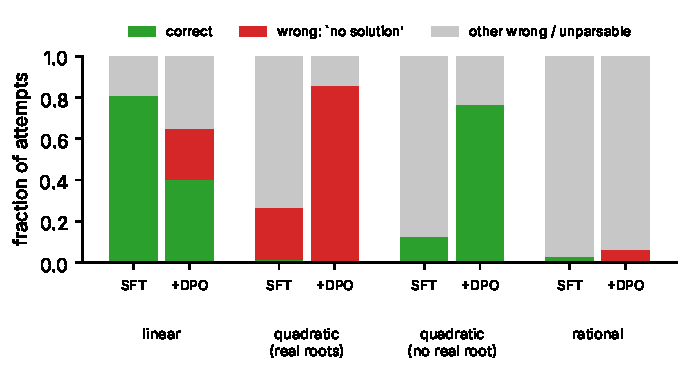
\includegraphics[width=0.62\linewidth]{figures/fig_displacement.pdf}
\caption{Outcome composition before (SFT) and after DPO, eight passes pooled. Red:
answered \nosol{} where a real root exists. DPO's apparent quadratic gain is confined to
quadratics without a real root, where \nosol{} is correct.}
\label{fig:displacement}
\end{figure}

\begin{figure}[t]
\centering
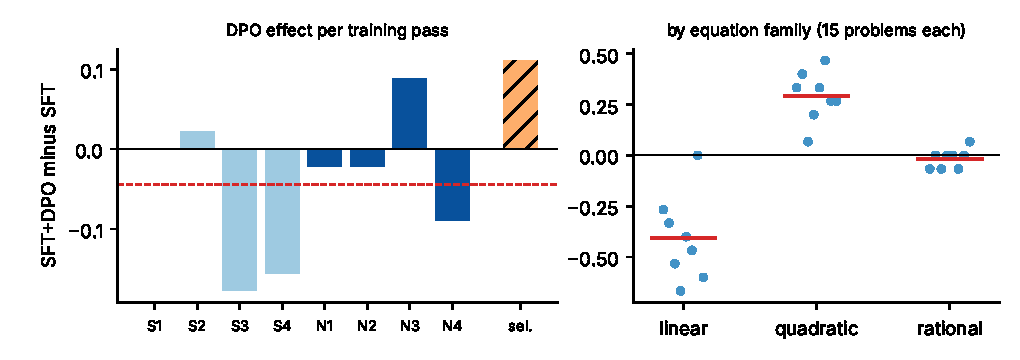
\includegraphics[width=0.9\linewidth]{figures/fig_dpo_passes.pdf}
\caption{Left: DPO effect (SFT+DPO minus SFT) in each of the eight training passes (S =
September, N = November) and the separately selected checkpoint (hatched); dashed line is
the eight-pass mean. Right: the same effect by equation family, one point per pass.}
\label{fig:dpo}
\end{figure}

\paragraph{A fix, not yet tested.}
We rebuilt the preference data so that \nosol{} occurs equally often on both sides:
the 25 no-real-root problems are restored with a plausible spurious root as the
rejected answer (the vertex $-b/2a$ for a quadratic, the excluded point for a rational
equation), and 25 solvable problems, stratified by family, are added with \nosol{} as
the rejected answer (168 pairs in total; the original 118 are a subset). Our prediction
is that \nosol{} on solvable problems returns to near the SFT rate and that the family
pattern disappears. We have not yet trained on this data; the configuration and a
notebook to run it are released.

\section{Verifier feedback does not reliably beat re-sampling}
\label{sec:feedback}

Table~\ref{tab:ladder} reports the ladder on three checkpoints that differ widely in
greedy accuracy ($0.133$, $0.244$, $0.444$). On the first (the weakest, from a DPO pass
that had degraded), \texttt{diagnostic} and \texttt{actionable} feedback beat
re-sampling by $+0.081$ and $+0.067$. We originally reported these with sign tests
over 135 problem--seed units ($p{=}0.019$ and $0.035$). With the problem as the unit,
\texttt{diagnostic} gives $p{=}0.042$ unadjusted and $0.166$ after Holm correction; no
condition is significant.

On the two November checkpoints, the effect is gone. \texttt{diagnostic} is $-0.015$
and $-0.022$. \texttt{actionable} is $-0.089$ on the second checkpoint, significantly
\emph{worse} than re-sampling (Holm $p{=}0.035$), and $+0.007$ on the third. No
condition beats \texttt{retry} by more than $+0.007$ on either November checkpoint.
Pooling the two checkpoints with raw data, \texttt{diagnostic} is $+0.033$
(95\% CI $[-0.015, +0.081]$, Holm $p{=}0.58$). The separate agent-loop experiment agrees:
feedback minus control at a three-turn budget is $+0.074$ ($p{=}0.13$) on the first
checkpoint and $+0.007$ ($p{=}1.0$) on the second (Figure~\ref{fig:agent}).

The only checkpoint on which feedback looked useful was the weakest one
(Figure~\ref{fig:quality}). That fits an intuition stated before the replication (a
damaged model leaves more for feedback to recover) but three checkpoints cannot
establish a trend, and the most defensible summary is that we find no reliable benefit
of verifier feedback over re-sampling for this model. Re-sampling itself is strong: on
every checkpoint, the \texttt{retry} control gains $0.06$--$0.12$ over turn 1. The
re-sampling control is what keeps the comparison honest: reported on its own, the feedback
condition's improvement from turn 1 to turn 3 on the first checkpoint ($0.207\to0.341$)
looks like a self-refinement result.

\begin{figure}[t]
\centering
\begin{minipage}[t]{0.47\linewidth}\centering
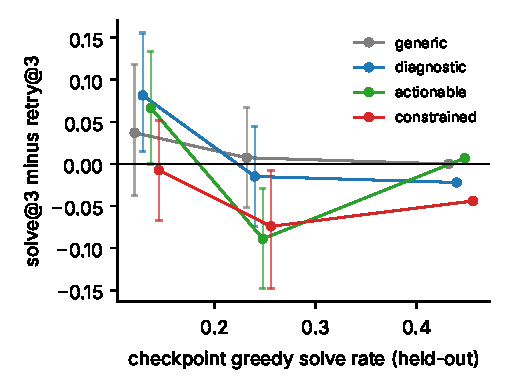
\includegraphics[width=\linewidth]{figures/fig_benefit_vs_quality.pdf}
\caption{Feedback minus re-sampling (solve@3) against the checkpoint's own greedy
accuracy. Error bars: problem-level 95\% bootstrap CIs (unavailable for the third
checkpoint, see \S\ref{sec:limits}).}
\label{fig:quality}
\end{minipage}\hfill
\begin{minipage}[t]{0.5\linewidth}\centering
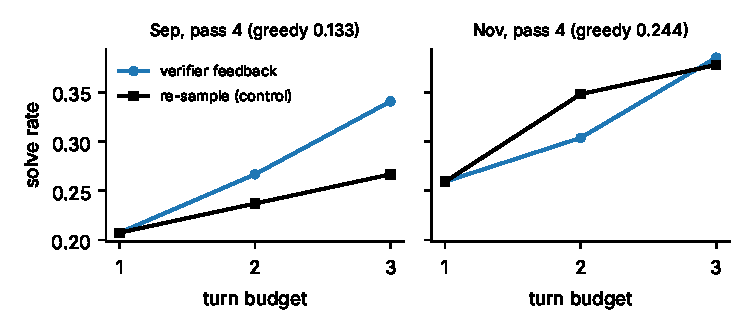
\includegraphics[width=\linewidth]{figures/fig_agent_loop.pdf}
\caption{Agent loop: cumulative solve rate by turn budget, verifier feedback vs.\ the
re-sampling control under identical sampling seeds, on two checkpoints. Turn budget 1 is
identical by construction.}
\label{fig:agent}
\end{minipage}
\end{figure}

\section{Feedback costs format validity, in proportion to prompt length}
\label{sec:format}

On all three checkpoints, the fraction of parsable answers falls in the same order as
the prompts get longer: \texttt{retry} ($0.91$, $0.94$, $0.96$ over all turns) $>$
\texttt{generic} ($0.82$, $0.87$, $0.88$) $>$ \texttt{diagnostic} ($0.78$, $0.85$,
$0.80$) $>$ \texttt{actionable} ($0.72$, $0.72$, $0.73$) $>$ \texttt{constrained}
($0.44$, $0.47$, $0.64$) (Figure~\ref{fig:format}). The \texttt{constrained} condition was
written to \emph{protect} the format by restating it, and it is the worst every time; at
turns 2--3 only $12\%$ (first checkpoint) and $14\%$ (second) of its answers were parsable. An
unparsable answer scores as wrong, so part of every feedback condition's deficit is
format, not reasoning. Our model was fine-tuned on a single prompt shape, which likely
makes it unusually sensitive to any deviation from it; whether the effect is as strong
for models trained on diverse prompts is open.

\begin{figure}[t]
\centering
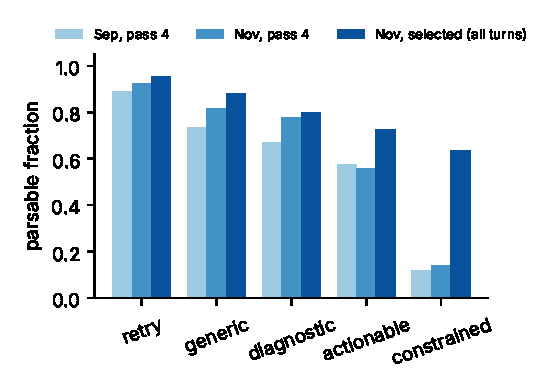
\includegraphics[width=0.5\linewidth]{figures/fig_format_validity.pdf}
\caption{Fraction of parsable answers by feedback condition (turns 2--3 for the two
checkpoints with raw data; all turns for the third).}
\label{fig:format}
\end{figure}

\section{Defects in our own pipeline}
\label{sec:defects}

Several of this project's earlier conclusions were wrong because of defects that
produced plausible numbers rather than errors. We list the ones that changed a
conclusion, because each is a failure mode other verifier-based pipelines can share.
\begin{itemize}
\item \textbf{The verifier rejected the format its own prompt demanded.} It accepted
\texttt{no solution} but not \texttt{x = no solution}, so correct answers on the 8
no-solution benchmark problems scored as unparsable, and the feedback loop told
correctly formatted answers to fix their format.
\item \textbf{A ``disjoint'' split was not disjoint.} A different random seed does not
produce a disjoint sample from a small space: 6 of 45 benchmark equations were in the
SFT data. Splits are now disjoint by construction and asserted.
\item \textbf{Hash-order nondeterminism.} Python's per-process string-hash salting made
``same seed'' produce different problem sets and, separately, different perturbed
answers for problems with irrational roots. Neither changed a solve rate (the verifier
compares sets), which is why they went unnoticed.
\item \textbf{The preference-data hole} of \S\ref{sec:dpo}, found by splitting an
aggregate by family.
\item \textbf{A synthetic result that confirmed its own premise.} An early CPU
experiment used a synthetic solver whose error rate was defined to fall with each turn,
and it was reported as showing that feedback helps. It showed only that the solver did
what it was programmed to do.
\item \textbf{Pseudo-replication.} The original ladder $p$-values treated seeds of one
problem as independent (\S\ref{sec:feedback}).
\end{itemize}
Three of these were found by writing tests that specify behaviour (which spellings the
verifier must accept; which datasets may overlap), after the code had been reviewed
line by line several times without finding them.

\section{Related work}

\paragraph{DPO failure modes.} DPO can reduce the likelihood of preferred
responses~\citep{pal2024smaug,feng2024limitations}, and \citet{razin2025displacement}
showed that the displaced probability can go to responses with the opposite meaning,
predicting it from the similarity of preferred and dispreferred responses. Our setting
is a small, fully checkable case of the same phenomenon in which the destination is a
single identifiable answer, and the cause is a gap in what the preference data
covers. \citet{tajwar2024preference} argue that preference fine-tuning benefits from
on-policy data; our rejected answers came from a synthetic error model rather than the
model itself, which is what made the coverage gap possible.

\paragraph{Self-correction.} Self-Refine~\citep{madaan2023selfrefine},
Reflexion~\citep{shinn2023reflexion} and CRITIC~\citep{gou2024critic} report gains from
feedback-driven revision. \citet{huang2024cannot} found that intrinsic self-correction
without external feedback does not improve reasoning, and \citet{kamoi2024survey} argue
that many reported gains lack fair baselines. Our study uses external, exact feedback,
which is the favourable case, and still finds no reliable gain over a re-sampling
baseline~\citep{brown2024monkeys} at this scale.

\section{Limitations}
\label{sec:limits}
One 0.5B model; three families of single-variable equations; 45 benchmark problems,
three sampling seeds per problem. The linear family has only 252 distinct equations.
Eight training passes give a reasonable picture of training variance, but only three
checkpoints were used for the feedback experiments, and for the third the per-attempt
rows were not preserved (they are inside a backup archive that also contains model
weights), so only point estimates are reported for it; the agent-loop run on that
checkpoint did not complete. The displacement mechanism is established for this
preference data; that balanced data removes it is a prediction we have not yet tested.
Our explanation of \emph{why} the mass goes to \nosol{} (similarity of rejected numeric
answers to correct ones) is a hypothesis consistent with the data, not a measured
mechanism.

\section{Conclusion}
With an exact verifier, two results that looked like progress turned out to be
something else. A DPO stage that appeared to fix quadratics had taught the model to say
\nosol{}, an answer its preference data never contained, while making correct answers
less likely. A feedback benefit measured on one checkpoint did not survive two more, or
a correct unit of analysis. The practical lessons are simple: check what preference data
\emph{does not} contain, not only that each pair is valid; break aggregate changes down
by answer, not only by score; compare refinement against re-sampling with paired seeds;
and replicate on more than one checkpoint before believing an inference-time gain.

\paragraph{Reproducibility.} Code, configurations, every raw generation behind every
number, the executed notebooks, and a 183-test suite (verifier verdicts, determinism
across interpreter processes, split disjointness, experiment validity, and agreement
between the documentation and the recorded numbers) are released.
\texttt{src/paper\_analysis.py} regenerates every table and figure in this paper on a CPU
in about 20 seconds.

\bibliographystyle{plainnat}
\bibliography{refs}

\end{document}
